\chapter{Architektur}

\section{Übersicht}

Um die beschriebenen Funktionalen- und Nicht-Funktionalen Anforderungen erfüllen zu können, haben wir die folgende Architektur entwickelt. \\

Um eine Drohne über einen Server in der Cloud steuern zu können, muss diese mit dem Internet verbunden werden. Um dies zu erreichen verwenden wir ein Smartphone, dass auf der Drohne angebracht wird und über USB mit dem Flight-Controller verbunden ist.  (siehe Abb. \ref{fig:architecture-overview}). Das Smartphone wird aber auch benötigt um dem Drone-Operator ein Benutzeroberfläche zur Verfügung zu stellen, die das Beladen und das Abfragen des Zustands der Drohne ermöglichen. \\

\begin{figure}[h]
	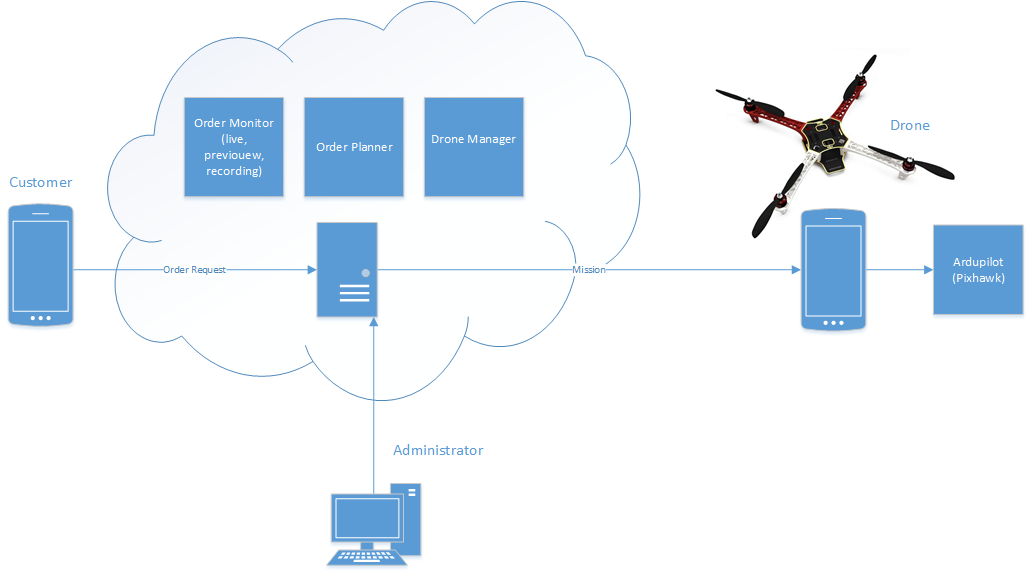
\includegraphics[width=1.0\textwidth]{images/Overview-Diagram.png}
	\caption{Übersicht der Project Helin Architektur }
	\label{fig:architecture-overview}
\end{figure}

\section{Kommunikations-Architektur}

Die Abbildung \ref{fig:communication-architecture-overview} zeigt die Kommunikations-Architektur in der Übersicht. Wichtig sind vor allem die verschiedenen verwendeten Protokolle, die benötigt werden um die Anforderungen erfüllen zu können. Bei den mobilen Geräten wird Messaging ({\Gls{AMQP}) verwendet, um bidirektionale Kommunikation zu ermöglichen. Dies ist nötig, damit Kunden und Administratoren die Bewegungen der Drohne live verfolgen können. Die eingesetzte Technologie für die Kommunikation zwischen dem Server und den Smartphones muss ausserdem den Nicht-Funktionalen-Anforderungen gerecht werden im Bezug auf Verbindungsabbrüche und Verbindungswiederherstellung.

\begin{figure}[h]
	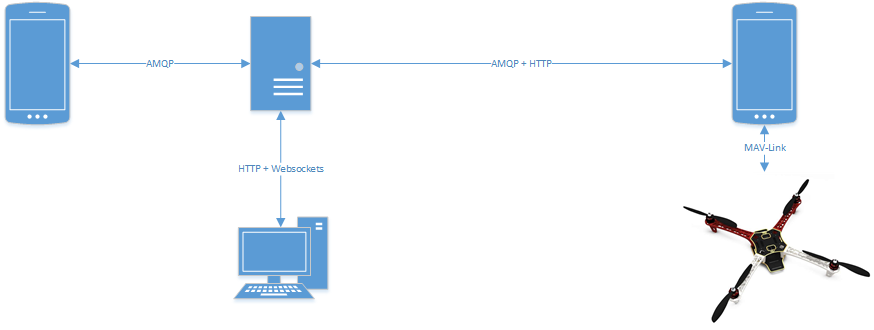
\includegraphics[width=1.0\textwidth]{images/Communication-Overview-Diagram.png}
	\caption{Übersicht der Kommunikations-Architektur mit den jeweiligen Protokollen. }
	\label{fig:communication-architecture-overview}
\end{figure}

\subsection{Verwendete Enterprise Integration Patterns}

Messaging-Systeme und -Protokolle bieten meistens eine grosse Auswahl an Patterns, die verwendet werden können. Für dieses Projekt benötigen wir nur einen kleinen Teil davon um die Anforderungen erfüllen zu können.

\subsubsection{Point-to-Point Channel}

Um zwischen einer registrierten Drohne und dem Server einen sicheren und zuverlässigen Nachrichtenaustausch zu ermöglichen, wird jede Drohne bzw. jede App über einen separaten Point-to-Point Channel angebunden, welcher ihr nach der Registrierung zugeteilt wird. Dies ermöglicht dem Server eine Nachricht nur an eine Drohne zu schicken.

\subsubsection{At-most-once delivery}

Wir müssen sicher sein, dass eine Drohne eine Mission oder einen Befehl nur ein Mal erhält. Ansonsten müsste Logik eingebaut werden, die diese Problematik löst. Sollte die Drohne einen Befehl oder eine Mission gar nicht erhalten, weil die Verbindung unterbrochen ist, muss das System dies wissen und entsprechend reagieren können.

\subsubsection{Event-driven Consumer}

Alle Aktoren des Systems müssen die Möglichkeit bieten auf Grund von Events bzw. Nachrichten Aktionen auszuführen. Beispielsweise:

\begin{itemize}
	\item Drohne erhält neue Mission vom Server und soll dies dem Drone-Operator anzeigen.
	\item Server erhält neue Position von der Drohne und soll diese Nachricht dem Kunden weiterleiten und dem Administrator auf dem Web-Client anzeigen.
	\item Smartphone des Kunden erhält neue Position der Drohne, auf der Karte wird die Position der Drohne angezeigt.
\end{itemize}
	
